        % Master Thesis Template for MSc Bioinformatics English
        % Prof. Daniel Huson, June 2025
        % Version 2.0
        \documentclass[12pt,a4paper]{report}

        % Packages
        \usepackage[utf8]{inputenc} % For UTF-8 encoding
        \usepackage[english, ngerman]{babel} % For English and German languages
        \usepackage{graphicx} % For including graphics
        \usepackage{amsmath, amssymb} % For math
        \usepackage{hyperref} % For hyperlinks
        \usepackage{geometry} % For page margins
        \usepackage{setspace} % For line spacing
        %\usepackage{natbib} % For author-year citations
        \usepackage[square,numbers]{natbib}
        \usepackage{titlesec} % Custom chapter heading format

        % Keep chapter numbering (shown in the table of contents) but drop the
        % "Chapter N" label line above the heading; the number stays inline as "N Title".
        \titleformat{\chapter}[hang]{\normalfont\huge\bfseries}{\thechapter}{1em}{}
        \titlespacing*{\chapter}{0pt}{0pt}{20pt}

        % Evaluation data and figures (exchangeable): every number is read from a single
        % CSV and every plot from one folder, so replacing those files updates the thesis
        % without touching the text. Change \plotdir if the files live elsewhere in Overleaf.
        \usepackage{datatool}
        \newcommand{\plotdir}{../plots}
        \graphicspath{{\plotdir/}}
        \DTLloaddb{evalresults}{\plotdir/eval_results.csv}
        % Fetch one evaluation value (or its unit) by its key from eval_results.csv.
        \newcommand{\evalval}[1]{\DTLfetch{evalresults}{key}{#1}{value}}
        \newcommand{\evalunit}[1]{\DTLfetch{evalresults}{key}{#1}{unit}}

        % Page setup
        \geometry{a4paper, margin=1in}
        \setstretch{1.5} % Line spacing

        %%%%%%%%%%%%%%%%%%

        % Title page information
        \title{\textbf{Title of the Thesis}}
        \author{Student's Full Name\\\\MSc Bioinformatics}
        \date{Month Year}

        %%%%%%%%%%%%%%%%%%
        \begin{document}
        %%%%%%%%%%%%%%%%%%

        \selectlanguage{english}

        %%%%%%%%%%%%%%%%%%
        % Note: this following outline is just a suggestion. Please rename chapters and sections to make them more specific, or
        % add and remove chapters or sections in which ever way is helpful.
        %%%%%%%%%%%%%%%%%%

        \begin{titlepage}
        \begin{center}
        {\LARGE University of Tübingen}\\\\
        {\large Faculty of Science \\
        Institute for Computer Science\\\\[4cm]}
        {\huge Master Thesis Computer Science\\\\[2cm]}
        {\Large\bf Learning Personalized Touchscrolling Functions\\\\[1.5cm]}
        {Felix Dietrich}\\\\[0.5cm]
        \today\\\\[3cm]
        {\small\bf Reviewers}\\\\[0.5cm]
        \parbox{7cm}{\begin{center}{\large Name First Reviewer}\\\\
        (Bioinformatics)\\\\
        {\footnotesize Institute for Bioinformatics and\\\\ Medical Informatics\\\\
            University of T\"ubingen}\end{center}}\hfill\parbox{7cm}{\begin{center}
        {\large Name Second Reviewer}\\\\
        (Area of research)\\\\
        {\footnotesize Institute of second reviewer\\\\
            University of T\"ubingen}\end{center}
        }
        \end{center}
        \end{titlepage}

        % Title page

        \thispagestyle{empty}
        \vspace*{\fill}
        \begin{minipage}{11.2cm}
        \textbf{Dietrich, Felix:}\\\\
        \emph{Title of thesis}\\\\ Master Thesis Computer Science\\\\
        University of T\"ubingen\\\\
        Thesis period: 01.05.2026 -- 31.10.2026
        \end{minipage}
        \newpage

        %%%%%%%%%%%%%%%%%%
        \chapter*{Abstract}






        %%%%%%%%%%%%%%%%%%

        \selectlanguage{english}
        \newpage

        %%%%%%%%%%%%%%%%%%
        \tableofcontents
        \newpage

        % Do not generate a list of figures

        % Do not generate a list of tables

        % Do not generate a list of abbreviations, please avoid using them, or keep reminding the user what they stand for.

        %%%%%%%%%%%%%%%%%%
        \chapter{Introduction}

        %%%%%%%%%%%%%%%%%%
        \chapter{Related Work}

        This chapter summarizes the literature relevant to the thesis and is structured into two main parts. The first part covers transfer functions and their role in pointing and scrolling interaction, while the second part presents the probabilistic machine learning background, including active learning and Gaussian processes. The goal is to provide the conceptual basis for the methods developed in this work.

        \section{Transfer Functions}

        \subsection{Fundamentals}

        Transfer functions map movements in the control space to movements in the display space. In order for this relationship to be meaningful, it must be hardware-independent. All movements must be expressed using standard length and time units such as meters and seconds, not device-specific ones such as Pixels~\cite{casiez2011no}. In the simplest case of a linear relationship, the scale factor between the two spaces is referred to as the Control-Display (CD) gain:

        \begin{equation}
            \text{CD gain} = \frac{V_{\text{display}}}{V_{\text{control}}}
        \end{equation}

        For this coefficient to be unit less, numerator and denominator must be expressed using the same length and time units~\cite{casiez2011no}. Whether static or dynamic, CD gain settings involve a trade-off between gross and fine positioning. High gains reduce the time required to approach a distant target but make it difficult to precisely position the cursor on it. Conversely, low gains support precise positioning but increase the time needed to cover large distances~\cite{mackenzie1995input}. This trade-off is commonly formalized by Fitts' law, which predicts the movement time $MT$ required to acquire a target as a function of the movement distance $D$ and target width $W$. Using the Shannon formulation, the model is given by
        \[
        MT = a + b\,\log_2\!\left(\frac{D}{W} + 1\right),
        \]
        where $\log_2\!\left(\frac{D}{W} + 1\right)$ denotes the index of difficulty
        and $a$ and $b$ are empirically determined constants \cite{mackenzie1992fitts}. The control-display (CD) gain may be constant or dynamically adjusted during an interaction. For example, it can be defined as a function of instantaneous movement velocity in the control space \cite{casiez2011no}. Conceptually, transfer functions can be decomposed into three transformations~\cite{quinn2012exposing, quinn2013touch}. First, translation converts device units such as degrees of rotation, millimeters of finger displacement, or force values into units meaningful to the system, such as pixels or lines. Users may be able to adjust this translation through device controls or system preferences. Second, a gain function amplifies or attenuates the input signal for example, to allow slow precise control when the device is manipulated slowly, and accelerated output when it is manipulated more aggressively. The gain level can be user-configurable in some cases. Third, a persistence component preserves a history of prior inputs and computed parameters such as velocity and acceleration, enabling time-dependent effects such as cumulative gain increases, inertia, or simulated friction. Data from this component can feed back into both translation and gain. Not all of these transformations need to be present in any given transfer function some may be absent, combined, or applied multiple times at different levels of the system stack, for instance when gain is applied both by a driver and again by a UI toolkit~\cite{quinn2012exposing}. This model applies equally to mouse-based pointing and scrolling as well as to touch-based scrolling. Despite their fundamental role in interaction, transfer functions are typically embedded as black boxes in proprietary operating system drivers and are not publicly documented~\cite{quinn2012exposing, quinn2013touch}. This creates three recurring problems for researchers. First, it restricts researchers' knowledge of the transfer-function behaviour that is active on a given system. Second, it complicates the replication of experimental studies, because the exact function parameters may be unavailable, undocumented, or difficult to reproduce across devices and operating systems. Third, undocumented transfer-function behaviour can interact with experimental conditions and thereby introduce unintended confounds into measured performance \cite{casiez2011no,quinn2012exposing}. Casiez and Roussel characterise this situation as a practice of bricolage. An unreflective patching together of conditions without precise knowledge of the transfer functions involved~\cite{casiez2011no}. Quinn et al.\ subsequently observed the same problems for scroll-wheel transfer functions~\cite{quinn2012exposing} and for touch scrolling transfer functions on smartphones and tablets~\cite{quinn2013touch}.

        \subsection{Pointing Transfer Functions}

        \subsubsection{Characterising and Replicating Commercial Functions}

        Indirect pointing has been the dominant interaction paradigm on desktop systems for decades. The mouse established itself as the primary input device after outperforming all other devices in early comparative studies on pointing speed and accuracy~\cite{casiez2011no}. In indirect pointing configurations, movements in the control space are mapped to movements in the display space. This mapping is referred to as a transfer function and must be defined in a hardware-independent manner. In the simplest case of a linear mapping, the control-display (CD) gain denotes the scale factor between the speed in the control space and the speed in the display space~\cite{casiez2011no}. Based on the hybrid optimized impulse motor control model, modern transfer functions typically apply high CD gains during the ballistic phase of a pointing movement, corresponding to high input velocities, and low CD gains during the corrective phase, corresponding to low input velocities~\cite{eddy2026tftune}. Despite their widespread use, the concrete design of transfer functions in commercial operating systems has long been poorly understood. \citeauthor{casiez2011no} found that many authors in the literature use constant CD gains as a baseline condition but fail to describe them in sufficient detail to allow replication~\cite{casiez2011no}. Moreover, enforcing a hardware-independent transfer function in practice even a constant one is considerably challenging~\cite{casiez2011no}. To address this, \citeauthor{casiez2011no} developed EchoMouse, an electronic device for characterizing the transfer functions of any system, and libpointing, a toolkit for replicating and comparing the transfer functions used by Windows, OS~X, and Xorg~\cite{casiez2011no}. Using these tools, they showed that the transfer functions of all three systems are non-linear and cannot be approximated by simple low-order polynomials the OS~X functions in particular exhibit piecewise-defined curves, some featuring unexplainable singularities~\cite{casiez2011no}. In a controlled experiment, the default transfer functions of all three systems outperformed a constant CD gain by up to 24\,\% in movement time, with significant differences between systems depending on target size~\cite{casiez2011no}. Notably, none of the participants was subjectively able to perceive any difference between the three system functions~\cite{casiez2011no}.

        \subsubsection{Hardware Independence}

        A limitation shared by many system-level pointing transfer functions is that they are conventionally expressed in virtual units, such as pixels per input count, rather than in physical units of distance and speed. Hanada et al.\ \citeauthor{hanada2021relevance} point out that a transfer function defined in this manner can produce markedly different observable pointer behaviour when it is used with input or output devices of different resolutions. In their first controlled study, they compared an 800-CPI mouse paired with a 122-DPI display with a 1000-CPI mouse paired with a 93-DPI display. Although these hardware differences were relatively small, the configuration significantly affected pointing performance for several tested operating-system transfer functions. Consequently, the combination of transfer function and hardware can constitute a confounding variable in experiments that do not report both precisely \cite{hanada2021relevance}.

        As a remedy, Hanada et al.\ demonstrate the applicability of hardware-independent transfer functions expressed in physical units. They propose two methods for preserving equivalent pointer behaviour on operating systems that require hardware dependent definitions: first, scaling a baseline function to the resolutions of the connected input and output devices; second, selecting the available operating system acceleration setting whose behaviour most closely matches the intended physical behaviour. In a second experiment, the authors evaluated mouse resolutions of 400, 800, 1600, and 3200 CPI in combination with display densities of 87 and 122 DPI. The resulting scaled and closest transfer functions yielded equivalent pointing performance across the tested hardware configurations, except in cases where the available operating-system settings could not provide a sufficiently close match. The authors additionally provide tools for computing equivalent transfer functions between hardware setups, supporting both consistent pointer behaviour for users and the replication of experimental conditions by researchers\cite{hanada2021relevance}.

        The practical importance of these software-level factors is underlined by work on touchpads, which have received far less attention than mice despite being the de facto standard input device on laptops. \citeauthor{an2025libpad} note that touchpad user experience is frequently reported to differ across operating systems. Apple's trackpads are widely regarded as superior but the underlying reasons have remained scientifically unexamined, as prior work focused mainly on hardware factors such as surface friction and physical size~\cite{an2025libpad}. To isolate the software contribution, they present LibPad, a toolkit that applies OS-specific transfer functions to arbitrary hardware, and reverse engineer the undocumented macOS touchpad function using a private multi-touch framework together with a Fitts'-law pointing task~\cite{an2025libpad}. Unlike mice, which report relative motion counts, touchpads report absolute coordinates and must therefore map input within a bounded surface area, which further couples the function to the device geometry~\cite{an2025libpad}. Their measurements reveal significant performance differences both across different laptop hardware running an identical transfer function and within the same hardware under different function configurations. That demonstrates that the transfer function and the physical touchpad both shape the perceived quality of touchpad pointing~\cite{an2025libpad}.

        Because the effective transfer function experienced by a user is thus the product of device firmware, driver, and operating-system settings, achieving a consistent mapping across environments is difficult. \citeauthor{kim2025hardware} address this by moving the mouse pointing transfer function into the device firmware itself. Their hardware-embedded approach lets users define a desired function in physical units on the device and then cancels out the influence of the OS-native function and of hardware setting perturbations, so that the uploaded function persists regardless of the operating system or hardware on which the device is used~\cite{kim2025hardware}. Motivated in part by competitive gaming, where consistent aiming behavior across machines is critical, their technical evaluation across transfer functions of various shapes shows robustness and accuracy comparable to the conventional, operating-system-side approach while removing the dependence on external configuration~\cite{kim2025hardware}.

        \subsubsection{Automatic and Personalised Optimisation}

        Although velocity-dependent transfer functions are known to outperform constant gains, their design has historically relied on manual trial and error or heuristic iteration~\cite{lee2020autogain}. AutoGain~\cite{lee2020autogain} introduced the first method to automatically optimize a gain function from a user's actual motion data, based on the assumption that the aiming error of individual submovements serves as an indicator of the inadequacy of the current gain function. If a submovement undershoots its intended aim point, the gain is too low and should be increased, if it overshoots, the gain is too high and should be decreased~\cite{lee2020autogain}. AutoGain segments each pointing movement into submovements based on local extrema in the speed profile and updates the gain function after each target acquisition trial proportionally to the measured aiming error for the respective speed ranges used~\cite{lee2020autogain}. In a study using a MacBook trackpad, AutoGain produced a gain function after approximately 30 minutes of active use that was comparable in performance to the manually tuned macOS function, a function that had been refined since 1994~\cite{lee2020autogain}. However, AutoGain was not able to significantly outperform existing OS transfer functions~\cite{eddy2026tftune}. TFTune addresses this limitation through a reinforcement learning based approach for automatically personalizing transfer functions. The tuning process is formulated as a Markov Decision Process in which the agent maps the current input magnitude to a coninuous gain value and receives a reward signal based on the achieved throughput achieved at the end of each trial~\cite{eddy2026tftune}. After training, the optimized policy is exported as a discrete lookup table and deployed as the final transfer function~\cite{eddy2026tftune}. Across three evaluation studies, TFTune demonstrated the ability to both create transfer functions from scratch and improve upon pre-established ones. On a MacBook trackpad, it outperformed the macOS default by 7\,\% in movement time within 7 minutes of tuning, and on participants' own Windows devices with varying hardware, an 8\,\% improvement was achieved in as little as one minute~\cite{eddy2026tftune}. After two to four weeks of real-world daily use, no perceived degradation was reported and all participants chose to retain their personalized functions~\cite{eddy2026tftune}. Unlike AutoGain, which adjusts individual speed bins locally, TFTune optimizes the transfer function as a parameterized policy, yielding smoother and more monotonic functions that generalize better across unseen input speeds~\cite{eddy2026tftune}.

        \subsection{Scrolling Transfer Functions}

        Although touchscreens had already been gaining traction at the time, \citeauthor{casiez2011no} anticipated that indirect pointing would remain the prevailing paradigm for the foreseeable future. This assumption has since been challenged by the rapid proliferation of mobile devices. As a result, touch-based scrolling, rather than mouse or trackpad interaction, has become the dominant mode of content navigation for a large share of users, making the design and understanding of touch scrolling transfer functions an increasingly critical concern. 

        \subsubsection{Input Parameters and the Scrolling Design Space}

        A scrolling transfer function can attend to a range of input parameters derived from how users physically interact with the device. These can be classified into three types. Instantaneous measures capture physical properties sensed at a given moment or their derivatives, such as angular velocity or acceleration of a scroll wheel, which can be used to increase scroll magnitude or switch between scrolling modes. Action duration refers to how long an input is sustained or absent, for instance, if scrolling velocity is maintained above a threshold, gain might increase on the assumption that the user intends to travel a long distance. Cumulative and relative inputs introduce memory of prior actions, such as cumulatively adding gain across rapidly repeated wheel rotations in the same direction, canceled if the user pauses or reverses direction~\cite{quinn2012exposing}.

        The design space available to a scrolling transfer function is closely tied to the physical characteristics of the input device and the limited mechanics of scroll control. \citeauthor{quinn2012exposing} organise these characteristics by drawing on established input-device taxonomies that classify controls by whether they sense position, motion, or force, along how many linear or rotational dimensions, and whether they operate in absolute or relative terms~\cite{quinn2012exposing}. This framing highlights why scrolling is comparatively impoverished as an input channel. While a modern mouse registers thousands of counts per inch across a two-dimensional area that can be traversed without clutching, a typical scroll wheel offers only five or six detents across roughly forty degrees of one-dimensional rotation between clutching actions, and the muscle groups involved impose asymmetric control capabilities across scroll directions~\cite{quinn2012exposing}. Because of this paucity of expressiveness, scrolling functions are likely to attend to several input parameters at once. The rate of device movement, the time between clutched repetitions, and the scroll direction among them, rather than to velocity alone as in pointing~\cite{quinn2012exposing}. To determine which of these parameters commercial systems actually use, and how, \citeauthor{quinn2012exposing} extend the EchoMouse and libpointing approach so that simulated input can be injected at controlled speeds and the resulting system response inspected, turning otherwise opaque driver behavior into measurable transfer functions~\cite{quinn2012exposing}. 

        \subsubsection{Reverse Engineering Commercial Scrolling Functions}

        Despite this rich design space, existing scrolling transfer functions are typically black boxes embedded in proprietary OS drivers, making them difficult to examine, report, or replicate~\cite{quinn2012exposing}. \citeauthor{quinn2012exposing} adapted the EchoMouse approach of Casiez and Roussel~\cite{casiez2011no} to reverse engineer the scrolling transfer functions of Apple Mac OS~X, Microsoft Windows~7, Microsoft IntelliPoint, and Logitech drivers~\cite{quinn2012exposing}. Their analysis revealed substantial variation across drivers. Neither Windows~7 nor Logitech's SetPoint provide any scroll acceleration (constant gain only), while Mac OS~X applies velocity-dependent gain using a smoothing window of the last eight events to avoid rapid gain changes, and IntelliPoint cumulatively adds gain across successive clutch actions~\cite{quinn2012exposing}. Notably, Mac OS~X exposes a Scrolling Speed slider to users via eight intervals mapped to API values from 0 to 1.7, where a negative value completely disables acceleration for generic devices, or engages a page-scrolling mode for Apple trackpads~\cite{quinn2012exposing}. While scroll-wheel transfer functions can be examined through HID-based methods, touch scrolling presents additional complexity~\cite{quinn2013touch}. While Android's scrolling code is publicly available as open source, Apple and Microsoft require indirect approaches, either programmatic control of the iOS simulator with subsequent replay on an actual device, or decompilation of bytecode in Microsoft's case~\cite{quinn2013touch}.

        Regarding the transfer functions themselves, both iOS and Android maintain a 1:1 mapping between finger movement and scrolling output while the finger remains in contact with the display~\cite{quinn2013touch}. Once the finger leaves the surface, however, both systems can substantially amplify the output, applying cumulative gain to assist users in traversing long distances~\cite{quinn2013touch}. The two systems differ in how this gain is applied. iOS applies a capped velocity multiplier after the fourth successive flick gesture (with the cap reaching 16 from the tenth gesture onward), while Android continuously adds any residual scroll velocity to the next flick without an upper cap~\cite{quinn2013touch}. Both systems also apply simulated friction to progressively retard scroll velocity after the finger lifts, with iOS using an exponential decay model and Android relying on spline-based deceleration curves~\cite{quinn2013touch}. \citeauthor{quinn2013touch} believe, that these findings highlight several opportunities for improving touch scrolling transfer functions. Since clutch time is a reliable signal of scroll intent, it could be explicitly incorporated as a parameter in gain functions to enable accelerated scrolling across repeated gestures. Furthermore, document-length-dependent gain, which uses a 1:1 mapping at slow input rates but scales gain according to document length at high rates has been identified as a particularly promising approach for mobile devices with small viewports and long content~\cite{quinn2013touch}.

        Reverse engineering touch scrolling required different tools than those used for scroll wheels, because touch input cannot be injected through the published USB standards that HID-based methods rely on~\cite{quinn2013touch}. \citeauthor{quinn2013touch} therefore combined controlled software simulation with a high-precision Selective Compliant Articulated Robot Arm (SCARA) that mechanically reproduces touch scrolling gestures with repeatable length and velocity, allowing the black-box functions of commercial devices to be probed directly on the hardware~\cite{quinn2013touch}. Alongside this system-side analysis, they conducted a human-factors experiment to characterise how users actually express scrolling intentions through touch gestures, establishing the practical limits and variability of gesture velocity, length, and repetition that a transfer function must accommodate~\cite{quinn2013touch}. This pairing of a human-behavior study with a device-measurement method is important because it grounds the observed system behavior in the range of inputs users are able and likely to produce, rather than in idealised gestures~\cite{quinn2013touch}. Applying the method to Apple iOS on both iPhone and iPad and to Google Android, they found broad similarities but also substantial platform-specific differences, implying that any experiment involving gestural scrolling is liable to be influenced by the platform on which it is conducted. To support replication and iterative improvement, they released the extracted data tables and the software used to emulate and test the functions~\cite{quinn2013touch}.



        \subsubsection{Modelling and Evaluating Scrolling Performance}

        A foundational step toward rigorous evaluation of scrolling techniques was made by \citeauthor{hinckley2002quantitative}, who proposed a formal experimental paradigm based on Fitt's Law. While Fitts' Law had traditionally been applied to pointing tasks involving rapid, aimed movement to visible targets, their work demonstrated that it also models scrolling performance well, despite the scrolling target lying beyond the edges of the screen. Their paradigm systematically varies two parameters, scrolling distance and required tolerance. Applying this paradigm to two representative devices, the IBM ScrollPoint isometric joystick and the Microsoft IntelliMouse wheel, revealed a crossover effect in performance as a function of distance. The wheel was faster for short scrolling distances of up to roughly one hundred lines, whereas the isometric joystick became faster for longer distances~\cite{hinckley2002quantitative}. This result is methodologically significant, because a study that reports only overall means, without controlling for distance and tolerance, can reach opposite conclusions depending on the particular distances sampled~\cite{hinckley2002quantitative}. \citeauthor{hinckley2002quantitative} further showed that adding an acceleration algorithm substantially improved the wheel. At a high resolution of one line per notch it matched or exceeded the joystick up to about two hundred lines, and at three lines per notch up to about four hundred lines, demonstrating that scroll acceleration can extend the effective range of an otherwise short-range device~\cite{hinckley2002quantitative}. To date, no ISO standard equivalent to ISO~9241-9 exists for scrolling. 

        \citeauthor{zhao2014model} argue that scrolling on touch screens lacked a sufficiently solid theoretical basis, which made it difficult to compare techniques, model user performance, and predict interaction outcomes \cite{zhao2014model}. To address this gap, they do not treat scrolling as a single monolithic action, but first decompose it through a pilot study and task analysis into a simplified target-acquisition problem \cite{zhao2014model}. The authors model 1D scrolling as a two-phase process, consisting of an iterative searching phase followed by a conventional pointing phase once the target becomes visible \cite{zhao2014model}. This decomposition is important because it captures the fact that off-screen target acquisition on touch devices requires an unknown number of repeated pan or flick actions, unlike earlier one- or two-stage pointing paradigms that can largely be described with Fitts' law alone \cite{zhao2014model}. In other words, the study is designed to isolate the repeated clutch-like behavior that characterizes real touch scrolling, rather than collapsing it into a single pointing movement \cite{zhao2014model}. The experiment itself was intentionally constrained to a horizontal 1D setting, with the display window, workspace, target distance, display size, and target width manipulated systematically \cite{zhao2014model}. The authors further separated the interaction into two scrolling modes, panning and flicking, and two feedback conditions, with and without distance feedback, yielding four techniques in total \cite{zhao2014model}. This design choice allowed them to study not only whether scrolling performance differs across techniques, but also how target information and control mode shape the structure of the task \cite{zhao2014model}. Methodologically, the pilot study served to justify the simplifying assumptions used in the model. Repeated clutches during search, similar finger-displacement distributions across iterations, a ceiling effect on displacement, and an unknown starting position for the final pointing step \cite{zhao2014model}. The authors then formalize these observations into a quantitative model and validate it experimentally, showing that their task decomposition is not merely descriptive but directly supports the mathematical structure of the model \cite{zhao2014model}. Importantly, they also note that their experimental conditions represent useful extremes, while practical interfaces likely lie somewhere between these boundary cases \cite{zhao2014model}.

        From the four assumptions, \citeauthor{zhao2014model} derive a closed-form movement-time model whose central components correspond to the iterative search and the final pointing phase, and they validate both the complete model and its individual components against the experimental data~\cite{zhao2014model}. Beyond the conventional coefficient of determination $R^2$, they compare their model with existing models of related tasks using the Akaike Information Criterion, which balances goodness of fit against model complexity, and report that their formulation performs best under both criteria~\cite{zhao2014model}. The analysis further shows that panning and flicking shape the searching phase in different ways. Distance feedback generally improves scrolling performance, although its effects depend on the target distance, display-window size, and scrolling mode~\cite{zhao2014model}. The authors situate scrolling within the broader significance of the task, citing earlier observations that users may spend on the order of forty minutes merely scrolling during a multi-hour browsing session, so that even small efficiency gains accumulate into meaningful benefits~\cite{zhao2014model}. As a design implication, the model provides a principled basis for comparing and predicting the performance of direct-touch scrolling techniques and offers a foundation on which more sophisticated scrolling interactions can be modelled quantitatively~\cite{zhao2014model}.

        \subsubsection{Synthesis and Research Gap}

        Taken together, this body of work reveals a consistent trajectory. Early efforts established that transfer functions are pervasive yet poorly documented and introduced tools to characterise and replicate them~\cite{casiez2011no, quinn2012exposing, quinn2013touch}. Subsequent work quantified how strongly the function, the hardware, and the operating system jointly determine performance~\cite{hanada2021relevance, an2025libpad, kim2025hardware}. The most recent contributions turn from characterisation to optimisation, using automated and learning-based methods to tune functions to individual users~\cite{lee2020autogain, eddy2026tftune}. For touch scrolling in particular, however, the transfer functions of commercial platforms remain hand-tuned black boxes, and no comparable method exists for automatically adapting them to individual users or content. The gap that this thesis addresses.

        \section{Related Work: Machine Learning}

        \subsection{Problem Setting: Learning with a Goal}
        A recurring theme across active learning, Bayesian optimization, and related goal-driven methods is sample efficiency. The goal is to obtain the largest possible gain in knowledge or objective value from as few expensive evaluations as possible. Di Fiore et al.~\cite{di2024active} survey these fields from a unified perspective and describe the common pattern in which a probabilistic surrogate model and a selection criterion are combined iteratively to decide where the next informative measurement should be taken. This viewpoint is relevant whenever each evaluation carries a substantial cost, so that the efficiency of the search process matters as much as the quality of the final solution \cite{di2024active}.

        The unifying abstraction underlying these methods is adaptive sampling. Instead of drawing evaluation points from a fixed, predetermined design, the location of the next observation is chosen adaptively based on everything that has been learned so far \cite{di2024active}. Formally, one maintains a dataset $\mathcal{D}_t = \{(x_i, y_i)\}_{i=1}^{t}$ of already evaluated inputs $x_i$ and their (possibly noisy) responses $y_i$, fits a probabilistic model to $\mathcal{D}_t$, and derives from that model a scalar utility which is called an infill criterion in the design-of-experiments literature and an acquisition function in bayesian optimisation that ranks every candidate point by its expected usefulness \cite{di2024active}. Maximizing this utility yields the next query $x_{t+1}$, its response is observed, the model is updated, and the loop repeats until an evaluation budget is exhausted. Di Fiore et al.~\cite{di2024active} show that active learning and bayesian optimisation are two instances of this same symbiotic template that differ mainly in what usefulness means. Active learning seeks points that most improve the surrogate model itself, whereas bayesian optimisation seeks points that most improve the optimization objective.

        This distinction matters because it clarifies why Gaussian processes appear in both fields and why techniques developed in one can often be transferred to the other \cite{di2024active}. The survey further distinguishes between searches informed by a single information source and searches that exploit multiple levels of fidelity, where cheaper but less accurate approximations of the objective are combined with rare, expensive high-fidelity evaluations \cite{di2024active}. In all of these variants, the central design decision is the selection criterion, because it alone determines how a limited budget of costly evaluations is allocated across the search space. The remainder of this section therefore builds up the required background in the order in which it is needed. Supervised learning as the modelling foundation, active learning and BO as the two goal-driven sampling paradigms, Gaussian processes as the surrogate model that couples them, and acquisition functions as the decision rule that governs the tradeoff betwenn exploitation and exploration.

        \subsection{Supervised Learning}
        Supervised learning is the setting in which a model is trained on labeled input and output pairs and learns a mapping. The learner is given a training set $\{(x_i,y_i)\}_{i=1}^{n}$ and should learn a function that performs well not only on the training examples but also on previously unseen inputs. This ability is referred to as generalization \cite{Goodfellow-et-al-2016}. Depending on the nature of the target variable, the task is usually formulated either as classification, where the label is discrete, or as regression, where the label is continuous \cite{nasteski2017overview}.

        Nasteski~\cite{nasteski2017overview} reviews several supervised-learning methods, including decision trees, naive Bayes, linear and logistic regression, support vector machines, nearest-neighbour methods, and neural networks. The overview discusses their basic principles and illustrates their use for different prediction problems and application contexts \cite{nasteski2017overview}. The choice of model class and training procedure influences which solutions are preferred among models that fit the observed data. For example, regularization can impose constraints or express a preference for simpler model classes in order to promote generalization \cite{Goodfellow-et-al-2016}.

        A model with excessive capacity may fit the training data too closely and memorize the training set, resulting in poor generalization to new inputs. This phenomenon is known as overfitting \cite{Goodfellow-et-al-2016}. More generally, training minimizes the empirical risk on a finite training set, whereas the desired objective is a low expected error over the underlying data-generating distribution. If the available training data do not adequately reflect the regions relevant for later predictions, a model may therefore achieve a low training error while still generalizing poorly \cite{Goodfellow-et-al-2016}.

        \subsection{Active Learning}
        Active learning extends the supervised setting by allowing the learning algorithm to choose which unlabeled instances should be labeled next, rather than relying on a fixed training set. Instead of passively accepting the available training data, an active learner iteratively identifies the most informative candidates and requests their labels from an oracle, which is particularly useful when labeled data are scarce, expensive, or time-consuming to obtain \cite{settles2009active}. For the same labeling budget, a learner can produce better models if it selectively queries the most informative data points \cite{settles2009active}.

        Settles \cite{settles2009active} organizes the field along the two the scenario in which queries are posed and the strategy by which their informativeness is quantified. Three canonical scenarios are distinguished. In membership query synthesis the learner may request a label for any point in the input space, including artificially constructed inputs that may not correspond to any natural instance. In stream-based selective sampling unlabeled instances arrive one at a time and the learner decides on the fly whether to query or discard each one. In pool-based active learning, the most common scenario in practice, a large pool of unlabeled instances is available at once and the learner ranks the entire pool to select the most informative query \cite{settles2009active}. The survey discusses several query-strategy frameworks \cite{settles2009active}:

        \begin{itemize}
            \item \emph{Uncertainty sampling} selects instances for which the
            current model is least certain about the label.

            \item \emph{Query-by-committee} selects instances on which the
            committee members disagree most.

            \item \emph{Expected model change} favors instances that are expected
            to alter the current model most strongly.

            \item \emph{Expected error or variance reduction} selects instances
            expected to reduce future prediction error or predictive variance.

            \item \emph{Density-weighted methods} combine informativeness with
            representativeness by down-weighting isolated outliers.
        \end{itemize}
        These frameworks differ in how they define informativeness. In particular, density-weighted methods explicitly combine uncertainty with representativeness, whereas other approaches focus primarily on model disagreement, model change, or expected future error \cite{settles2009active}.

        When Gaussian processes are used as the underlying model, the informativeness of a query is tied directly to the model's predictive uncertainty, because a GP provides both a predictive mean and a predictive variance at every candidate point rather than a single point prediction \cite{riis2022bayesian}. Riis et al.~\cite{riis2022bayesian} emphasize that the bias variance trade-off becomes more pronounced the less data are available. For GPs, the inferred predictive uncertainty depends substantially on hyperparameters such as the kernel length scale and the observation-noise term. They show that relying on a single point estimate of these hyperparameters can misrepresent the true predictive uncertainty and thereby mislead the query selection, whereas a fully Bayesian treatment that approximates the joint posterior over the hyperparameters yields more reliable uncertainty estimates and more efficient querying \cite{riis2022bayesian}.

        \subsection{Bayesian Optimization}
        Bayesian optimization models an unknown objective as a random function and selects the next evaluation point by maximizing an acquisition function \cite{snoek2012practical}. For expensive black-box problems it is especially attractive because it combines global search with explicit uncertainty management. Formally, Bayesian optimization addresses problems of the form $x^{\star} = \arg\max_{x \in \mathcal{X}} f(x)$ where $f$ is expensive to evaluate, possibly noisy, and provides no gradient information, so that classical gradient-based optimizers are inapplicable \cite{snoek2012practical}. Its two central components are a probabilistic surrogate model and an acquisition criterion that balances exploration and exploitation \cite{snoek2012practical}.

        The Bayesian optimization procedure follows the adaptive-sampling template
        introduced above and can be summarized as follows:

        \begin{enumerate}
            \item Given the current dataset $\mathcal{D}_t$, fit or update the
            Gaussian-process posterior.

            \item Construct the acquisition function $\alpha_t(x)$ from the current
            posterior.

            \item Optimize the acquisition function and select the next candidate
            \[
                x_{t+1} = \arg\max_{x \in \mathcal{X}} \alpha_t(x).
            \]

            \item Evaluate $x_{t+1}$ on the true objective function and observe
            \[
                y_{t+1} = f(x_{t+1}) + \varepsilon_{t+1}.
            \]

            \item Append the new observation to the dataset:
            \[
                \mathcal{D}_{t+1}
                =
                \mathcal{D}_t \cup \{(x_{t+1},y_{t+1})\}.
            \]

            \item Repeat the procedure until the evaluation budget is exhausted or
            another stopping criterion is reached.
        \end{enumerate}

        Because the acquisition function is substantially cheaper to evaluate than the true objective, its inner optimization can be performed before incurring the cost of the next objective evaluation. This separation between inexpensive candidate selection and expensive objective evaluation is central to the sample efficiency of Bayesian optimization~\cite{snoek2012practical,di2024active,balandat2019botorch}.

        \subsection{Gaussian Processes as Surrogate Models}
        A Gaussian process (GP) is a probability distribution over functions. It is
        defined by a mean function $m(x)$ and a positive-definite covariance function
        (or kernel) $k(x,x')$~\cite{williams1995gaussian,rasmussen2010gaussian}. We write
        \[
            f \sim \mathcal{GP}\bigl(m(x), k(x,x')\bigr).
        \]

        The defining property of a GP is that any finite collection of function
        values is jointly Gaussian. For inputs
        $X = \{x_1,\ldots,x_n\}$, the corresponding function values satisfy
        \[
            \mathbf{f}
            =
            \bigl(f(x_1),\ldots,f(x_n)\bigr)^\top
            \sim
            \mathcal{N}\bigl(\mathbf{m},K\bigr),
        \]
        where
        \[
            \mathbf{m}_i = m(x_i),
            \qquad
            K_{ij} = k(x_i,x_j).
        \]

        After observations have been incorporated, the GP defines a posterior
        distribution over functions. In particular, at a candidate point $x$ it
        provides a predictive mean $\mu(x)$ and a predictive variance
        $\sigma^2(x)$:
        \[
            f(x)\mid\mathcal{D}
            \sim
            \mathcal{N}\bigl(\mu(x),\sigma^2(x)\bigr).
        \]
        This predictive distribution supplies both a point prediction and a
        quantified measure of uncertainty, which is why GPs are useful as surrogate
        models in active learning and Bayesian optimization
        ~\cite{williams1995gaussian,rasmussen2010gaussian}.

        Concretely, given training inputs $X$ with observed targets $\mathbf{y}$ corrupted by independent Gaussian noise of variance $\sigma_n^2$, the predictive distribution at a test point $x_\ast$ is Gaussian with mean and variance
        \[
        \mu(x_\ast) = \mathbf{k}_\ast^{\top}\left(K + \sigma_n^2 I\right)^{-1}\mathbf{y}, \qquad
        \sigma^2(x_\ast) = k(x_\ast, x_\ast) - \mathbf{k}_\ast^{\top}\left(K + \sigma_n^2 I\right)^{-1}\mathbf{k}_\ast,
        \]
        where $K$ is the kernel matrix over the training inputs and $\mathbf{k}_\ast$ collects the covariances between $x_\ast$ and the training inputs \cite{williams1995gaussian,rasmussen2010gaussian}. These two quantities are precisely the $\mu(x)$ and $\sigma(x)$ consumed by the acquisition functions of the following section, which is why GPs are such a natural surrogate for Bayesian optimization.

        The covariance encodes assumptions about smoothness, length scales, and local variability across the search space \cite{williams1995gaussian,rasmussen2010gaussian}. Assigning a separate length scale to each input dimension additionally lets the model infer how strongly each variable influences the response \cite{rasmussen2010gaussian}. The kernel hyperparameters, together with the noise variance $\sigma_n^2$, are typically learned by maximizing the log marginal likelihood of the data, which automatically embodies a trade-off between data fit and model complexity \cite{rasmussen2010gaussian}. Williams and Rasmussen~\cite{williams1995gaussian} alternatively integrate over the hyperparameters using Hybrid Monte Carlo, which corresponds to the fully Bayesian treatment later emphasized for uncertainty-critical settings \cite{riis2022bayesian}.

        Efficient and numerically stable implementations of GP inference and hyperparameter learning are essential, because the required linear-algebra operations are cubic in the number of observations and can be ill-conditioned. Rasmussen and Nickisch~\cite{rasmussen2010gaussian} describe a modular GP toolbox that separates the choice of mean, covariance, and likelihood functions and relies on Cholesky factorization for stable evaluation of the marginal likelihood and its gradients.

        \subsection{Acquisition Functions for Exploration and Exploitation}
        Acquisition functions operationalize the sequential decision rule in Bayesian optimization. Rather than optimizing the expensive black-box objective $f(x)$ directly, Bayesian optimization maximizes a computationally inexpensive utility function $\alpha(x)$ derived from the current surrogate posterior \cite{snoek2012practical,balandat2019botorch}. The acquisition function therefore determines how Bayesian optimization trades off exploration of regions where the surrogate model is uncertain against exploitation of regions where the model predicts favorable objective values~\cite{shahriari2015taking}.

        The exploration exploitation trade-off is the central tension of any goal-driven sampling method. Pure exploitation risks becoming trapped near a local optimum, because it never tests regions the model currently underestimates. Pure exploration wastes the budget improving the model in regions that are irrelevant to the optimum. A good acquisition function resolves this tension by assigning utility to regions with high posterior uncertainty, favorable model predictions, or both \cite{shahriari2016taking}. For a minimization problem it generally favors candidates with low posterior mean $\mu(x)$, high posterior uncertainty $\sigma(x)$, or both, and the relative weight of these two quantities defines where a given criterion sits on the exploration exploitation spectrum \cite{di2024active,snoek2012practical}. The criteria surveyed below differ precisely in how they combine $\mu(x)$ and $\sigma(x)$, ranging from purely uncertainty-driven rules to improvement-based rules that adapt their exploratory behaviour to the current incumbent.

        \subsubsection{Probability of Improvement and Expected Improvement}
        Improvement-based acquisition functions select candidates according to their potential to improve upon a reference value. The probability of improvement (PI) considers only the probability that the latent objective value exceeds a specified target $\tau$. For a maximization problem, Shahriari et al.~\cite{shahriari2015taking} define
        \[
        \alpha_{\mathrm{PI}}(x;\mathcal{D}_n)
        :=
        \mathbb{P}\!\left[v(x)>\tau\mid\mathcal{D}_n\right]
        =
        \Phi\!\left(
        \frac{\mu_n(x)-\tau}{\sigma_n(x)}
        \right),
        \]
        where $\mu_n(x)$ and $\sigma_n(x)$ are the posterior mean and standard deviation, respectively, and $\Phi$ is the standard normal cumulative distribution function. In practice, the target $\tau$ may be chosen relative to the best value observed so far. Because PI treats all improvements beyond the target equally, it can behave greedily and concentrate evaluations near the current incumbent~\cite{shahriari2015taking}.

        Expected improvement (EI) remedies this by quantifying the expected magnitude of improvement over the best observed value \cite{jones1998efficient}. For noise-free maximization under the GP posterior it is defined as

        \[
        \alpha_{\mathrm{EI}}(x)
        =
        \underbrace{
        \left(\mu(x)-f^{+}\right)\Phi(z)
        }_{\text{exploitation}}
        +
        \underbrace{
        \sigma(x)\,\phi(z)
        }_{\text{exploration}},
        \qquad
        z=
        \frac{\mu(x)-f^{+}}{\sigma(x)}.
        \]
        where $\phi$ denotes the standard normal density and $\Phi$ its cumulative distribution function~\cite{jones1998efficient}. The first term is primarily associated with exploitation, as it rewards candidates whose posterior mean exceeds the incumbent value $f^{+}$. The second term captures the exploration effect of posterior uncertainty, since it increases with $\sigma(x)$ whenever an improvement remains plausible. The two terms are coupled through the standardized improvement $z$. Consequently, EI favors candidates that either have a high predicted value or retain sufficient uncertainty to plausibly improve upon the incumbent. It therefore provides an implicit exploration--exploitation trade-off without requiring a separate tunable trade-off parameter~\cite{jones1998efficient}.

        \subsubsection{Expected Improvement under Noise}
        When observations are noisy, the latent function value at the currently best observed configuration is not known exactly. Replacing this unknown incumbent with the best noisy observation or with a plug-in estimate based on the GP posterior mean can lead to unreliable decisions, particularly when the observation noise is large. In such settings, the incumbent estimate may be strongly affected by observation noise, and plug-in EI can exhibit overly exploitative behavior or insufficient exploration \cite{letham2019constrained}. Noisy expected improvement (NEI) addresses this issue by treating the latent function values at the previously evaluated configurations as uncertain and integrating the improvement utility over their joint posterior. For a maximization problem, let $\mathbf{f}=(f_1,\ldots,f_n)$ denote the latent function values at the observed configurations and define
        \[
        f^{+}(\mathbf{f}) := \max_{i=1,\ldots,n} f_i.
        \]
        The NEI acquisition function is then
        \[
        \alpha_{\mathrm{NEI}}(x\mid\mathcal{D})
        =
        \int
        \alpha_{\mathrm{EI}}\!\left(
        x\mid f^{+}(\mathbf{f})
        \right)
        p(\mathbf{f}\mid\mathcal{D})\,d\mathbf{f}.
        \]
        Thus, the incumbent is not fixed to a single noisy estimate; instead, it is
        sampled jointly with the latent function values from the posterior
        distribution \cite{letham2019constrained}. Marginalizing over this uncertainty
        avoids committing to a potentially misleading incumbent and yields a more
        robust estimate of the expected improvement. The resulting integral generally
        has no analytic closed form and is therefore approximated using Monte Carlo or
        quasi-Monte Carlo sampling \cite{letham2019constrained,balandat2019botorch}.

        \subsubsection{Monte Carlo Acquisition Functions}
        For many modern acquisition criteria, the relevant posterior expectation has no closed-form expression and is therefore approximated using Monte Carlo (MC) samples from the surrogate posterior. Wilson et al. \cite{wilson2018maximizing} show that a broad class of acquisition functions can be represented as the expectation of a utility function evaluated at posterior function values. For a candidate set $X$, a MC acquisition function can be written as
        \[
        \alpha_{\mathrm{MC}}(X)
        \approx
        \frac{1}{N}\sum_{i=1}^{N}
        u\!\left(\mathbf f^{(i)}(X)\right),
        \qquad
        \mathbf f^{(i)}(X)
        \sim
        p\!\left(\mathbf f(X)\mid\mathcal{D}\right),
        \]
        where $u$ denotes the utility function, such as an improvement over an
        incumbent. For a Gaussian-process posterior, the samples can be generated
        using the reparameterization
        \[
        \mathbf f^{(i)}(X)
        =
        \boldsymbol{\mu}(X)
        +
        L(X)\boldsymbol{\varepsilon}^{(i)},
        \qquad
        \boldsymbol{\varepsilon}^{(i)}\sim\mathcal{N}(\mathbf{0},I),
        \]
        with $L(X)L(X)^\top=\boldsymbol{\Sigma}(X)$. This representation makes the sample paths differentiable with respect to $X$ under suitable regularity conditions, allowing the MC acquisition function to be optimized using gradient-based methods \cite{wilson2018maximizing,balandat2019botorch}.

        For the class of myopic maximal acquisition functions considered by Wilson et al., the resulting batch objective is submodular. Consequently, greedy maximization admits near-optimality guarantees under the usual assumptions for normalized monotone submodular functions~\cite{wilson2018maximizing}.

        Building on this Monte Carlo framework, BoTorch implements parallel noisy expected improvement (qNEI). For a batch $X=(x_1,\ldots,x_q)$ and a set of baseline points $X_{\mathrm{base}}$, qNEI evaluates the expected improvement jointly under posterior samples at the new and baseline points:
        \[
        \alpha_{\mathrm{qNEI}}(X)
        =
        \mathbb{E}\left[
        \left(
        \max_{x\in X} f(x)
        -
        \max_{x'\in X_{\mathrm{base}}}f(x')
        \right)_+
        \middle|\mathcal{D}
        \right].
        \]
        Thus, qNEI avoids committing to a single deterministic incumbent and
        incorporates uncertainty in the latent objective values through the joint
        posterior \cite{balandat2019botorch}.

        \subsubsection{Numerically Stable Improvement: LogEI and qLogNEI}
        A practical difficulty of improvement-based acquisition functions is that their values and gradients can become numerically negligible over large regions of the search space. For Monte Carlo criteria, the sample-level improvement is zero whenever the sampled candidate batch does not improve upon the sampled incumbent. If this occurs for most or all posterior samples, the resulting Monte Carlo average and its gradient become numerically uninformative. This problem becomes more pronounced as the number of observations, the dimension of the search space, or the number of constraints increases \cite{ament2023unexpected}.

        Ament et al.~\cite{ament2023unexpected} attribute the inconsistent and often suboptimal empirical performance of EI and its variants, including constrained, parallel, and noisy forms, in part to these numerical optimization pathologies. They propose LogEI, a family of reformulations whose members have identical or approximately equal optima to their canonical counterparts while being substantially easier to optimize numerically. The reformulations evaluate positive improvement quantities in log-space and use stable smooth approximations for operations such as the sample-level maximum and constraint indicators. This preserves informative gradients in regions where the canonical implementations become numerically zero \cite{ament2023unexpected}.

        The family also includes qLogNEI, a numerically stable reformulation of parallel noisy expected improvement. qLogNEI smooths the sample-level improvement and feasibility operations and evaluates the resulting positive quantities in log-space. It therefore approximates the same underlying decision criterion as qNEI while generally providing more informative gradients and more reliable inner optimization \cite{ament2023unexpected}. For this reason, qLogNEI is used instead of canonical qNEI in this work.

        \subsubsection{Exploitation via the Posterior Mean}
        The acquisition functions above govern where to \emph{sample} next and therefore deliberately reward posterior uncertainty in order to explore regions the surrogate model has not yet resolved. Once the evaluation budget is exhausted, however, the procedure must return a single \emph{final recommendation}: the configuration reported as the estimated optimum. For this concluding decision exploration is no longer beneficial, because the reported point should reflect predicted performance rather than informativeness \cite{shahriari2015taking}. Continuing to use an exploration-driven acquisition function at this stage would risk recommending a candidate that is attractive only because it lies in an under-explored region, for example near the boundary of the search space, rather than because the model predicts it to perform well.

        A standard choice for the final recommendation is therefore the minimizer of the posterior mean (equivalently, the maximizer for a maximization objective),
        \[
        x^{\star}
        =
        \arg\min_{x\in\mathcal{X}}
        \mu(x),
        \]
        which corresponds to pure exploitation of the surrogate model: it selects the configuration that the fitted Gaussian process predicts to be best in expectation, ignoring the predictive uncertainty $\sigma(x)$ that the acquisition functions above deliberately reward \cite{shahriari2015taking,di2024active}. Because $\mu(x)$ is the smoothed posterior mean rather than an individual noisy observation, this criterion integrates information across all observed data and is robust to the noise in single evaluations, in contrast to simply returning the best observed point. In terms of the exploration--exploitation trade-off, the acquisition functions used during the optimization phase combine $\mu(x)$ and $\sigma(x)$, whereas the final recommendation relies on $\mu(x)$ alone.


        \subsection{BoTorch and PyTorch-based Bayesian Optimization}
        BoTorch is a modular Bayesian optimization framework built on PyTorch that provides particularly strong support for Monte Carlo acquisition functions, automatic differentiation, and hardware acceleration \cite{balandat2020botorch}. Its design reflects the fact that many modern acquisition functions can be expressed as expectations over posterior samples. Such estimators can be optimized efficiently when the complete computational graph is differentiable. BoTorch realizes this through sample average approximation (SAA). A fixed set of base samples is drawn once and reused during acquisition-function optimization, turning the Monte Carlo estimator into a deterministic objective conditional on those samples. This objective can then be optimized with deterministic gradient-based methods, including quasi-Newton methods such as L-BFGS-B \cite{balandat2019botorch}.

        Under stated regularity conditions, Balandat et al. \cite{balandat2019botorch} derive convergence results for the SAA estimators and their optimizers. The underlying differentiability of reparameterized Monte Carlo acquisition functions is also analyzed by Wilson et al.~\cite{wilson2018maximizing}. In practice, BoTorch provides three particularly relevant capabilities:
        \begin{itemize}
        \item modular abstractions for surrogate models, posterior samplers, objectives,
        and acquisition functions;
        \item gradient-based optimization of complex batch acquisition functions,
        enabled by automatic differentiation through reparameterized posterior
        samples; and
        \item support for parallel, asynchronous, noisy, and constrained optimization,
        together with randomized quasi-Monte Carlo sampling and efficient batched
        posterior evaluation
        ~\cite{balandat2019botorch,wilson2018maximizing}.
        \end{itemize}

        \chapter{Transfer Function Model}

        The transfer function governing fling motions is a physically motivated model derived directly from Android's OverScroller spline-deceleration algorithm.

        \section{Fling Phase}

        The fling phase is the normal, in-bounds momentum motion that follows a flick gesture. It is built on a strict separation between the scale of a fling (how far and how long it travels, computed from the launch velocity and a few constants) and its shape (the fixed, dimensionless temporal profile with which that distance is covered. Playback then simply stretches the shape onto the computed scale).

        \subsection{Scale: Physical Coefficient, Fling Distance, and Duration}

        The scale converts the launch velocity $v_0$ into a total travel distance $D$ and a total duration $T$. It relies on a device-specific physical coefficient
        \begin{equation}
        C \;=\; g \cdot 39.37 \cdot \mathrm{ppi} \cdot 0.84,
        \label{eq:sd-physical-coeff}
        \end{equation}
        where $g=9.80665\,\mathrm{m/s^2}$ and $\mathrm{ppi}$ is the display density in pixels per inch. Android does not hard-code this density but computes it at run time from the device metrics as $\mathrm{ppi}=160\,\rho$, where $\rho$ is the display-density factor (\texttt{OverScroller} line~640). Because the present study admits only iPhone devices, which all report the same density, this formula is replaced by the fixed value $\mathrm{ppi}=460$, so that $C$ is constant across participants rather than a device-dependent quantity. The scale further relies on a fixed dimensionless deceleration rate
        \begin{equation}
        r \;=\; \frac{\ln 0.78}{\ln 0.9} \;\approx\; 2.3582 .
        \label{eq:sd-decel-rate}
        \end{equation}
        Given a fling friction coefficient $\mu$, the distance and the duration (the latter in milliseconds) follow in closed form as
        \begin{align}
        D(v_0) &= \mu\,C \left( \frac{\beta\,\lvert v_0 \rvert}{\mu\,C} \right)^{\!\frac{r}{r-1}}, \label{eq:sd-fling-distance}\\[2pt]
        T(v_0) &= 1000 \left( \frac{\beta\,\lvert v_0 \rvert}{\mu\,C} \right)^{\!\frac{1}{r-1}}. \label{eq:sd-fling-duration}
        \end{align}
        Because $\tfrac{r}{r-1} > 1$ while $\tfrac{1}{r-1} < 1$, distance grows super-linearly and duration sub-linearly with $v_0$: a faster fling covers disproportionately more ground while spreading it over a comparatively shorter time.

        Table~\ref{tab:scale-params} collects these quantities together with their meaning and their origin in the \texttt{SplineOverScroller} inner class of Android's \texttt{OverScroller}. The scale is defined by three private methods: \texttt{getSplineDeceleration} returns the intermediate log term
        \begin{equation}
        L(v_0) \;=\; \ln\!\frac{\beta\,\lvert v_0\rvert}{\mu\,C},
        \label{eq:sd-spline-decel}
        \end{equation}
        which \texttt{getSplineFlingDistance} and \texttt{getSplineFlingDuration} feed into $\mu C\,e^{\frac{r}{r-1}L}$ and $1000\,e^{\frac{1}{r-1}L}$, respectively. Using the identity $\exp(a\ln z)=z^{a}$, these collapse to the closed forms of Equations~\eqref{eq:sd-fling-distance}--\eqref{eq:sd-fling-duration}. The fling scale uses Earth's gravity ($g=9.80665\,\mathrm{m/s^2}$), which is distinct from the private constant \texttt{GRAVITY}~$=2000$ used only for the separate edge/ballistic response.

        \begin{table}[htbp]
        \centering
        \begin{tabular}{l p{6cm} p{4.3cm}}
        \hline
        Symbol & Meaning & Source (line) \\
        \hline
        $v_0$ & Launch velocity (px/s) & input \\
        $g$ & Gravitational acceleration, $9.80665\,\mathrm{m/s^2}$ & \texttt{GRAVITY\_EARTH} \\
        $\mathrm{ppi}$ & Display density (px/inch); Android computes $160\,\rho$ at run time, here fixed to $460$ (iPhone only) so that $C$ is device-independent & constructor, 640 \\
        $C$ & Physical coefficient, Eq.~\eqref{eq:sd-physical-coeff} & \texttt{mPhysicalCoeff}, 641--645 \\
        $\mu$ & Fling friction (default $0.015$); scales distance and duration & \texttt{mFlingFriction}, 575 \\
        $r$ & Deceleration rate $\approx 2.3582$, Eq.~\eqref{eq:sd-decel-rate} & \texttt{DECELERATION\_RATE}, 586 \\
        $\beta$ & Inflexion factor ($0.35$) & \texttt{INFLEXION}, 587 \\
        $L(v_0)$ & Log deceleration term, Eq.~\eqref{eq:sd-spline-decel} & \texttt{getSplineDeceleration}, 783--785 \\
        $D(v_0)$ & Fling distance, Eq.~\eqref{eq:sd-fling-distance} & \texttt{getSplineFlingDistance}, 787--791 \\
        $T(v_0)$ & Fling duration (ms; factor $1000$), Eq.~\eqref{eq:sd-fling-duration} & \texttt{getSplineFlingDuration}, 794--797 \\
        \hline
        \end{tabular}
        \caption{Parameters and derived quantities of the fling scale, with their meaning and origin in the \texttt{SplineOverScroller} source.}
        \label{tab:scale-params}
        \end{table}

        \subsection{Spline Curve and Normalized Sampling}

        The scale provides the signed distance $D_s$ and the duration $T$. So that a single, fixed shape curve can describe every fling regardless of how far or how long it travels, these two quantities are normalized. Elapsed time is measured relative to $T$ and travelled distance relative to $D_s$, placing the motion in the dimensionless unit square $[0,1]\times[0,1]$. On this normalized domain the motion is a fixed position-versus-time spline $p(\tau)$ relating normalized time $\tau \in [0,1]$ to normalized distance $p \in [0,1]$. It is defined parametrically by two cubic B\'ezier curves sharing a common parameter $x \in [0,1]$; with the start and end tension constants $S = 0.5$ and $E = 1.0$ and the control ordinates
        \begin{equation}
        P_1 = S\,\beta = 0.175,
        \qquad
        P_2 = 1 - E\,(1-\beta) = 0.35,
        \label{eq:sd-control-points}
        \end{equation}
        the normalized time and distance are
        \begin{align}
        \tau(x) &= 3x(1-x)\big[(1-x)P_1 + x P_2\big] + x^3, \label{eq:sd-spline-time}\\
        p(x)    &= 3x(1-x)\big[(1-x)S + x\big] + x^3. \label{eq:sd-spline-pos}
        \end{align}
        This curve is sampled once, ahead of any fling and independently of $D_s$ and $T$, into a lookup table of $N+1 = 101$ entries ($N = 100$) holding $p$ at the equally spaced normalized times $\tau = i/N$.

        At run time this normalization is inverted to recover pixels. At elapsed time $t$ (ms) the duration $T$ normalizes time to $\tau = t/T \in [0,1]$, which indexes the table; the two surrounding entries yield the normalized position $p(\tau)$ and its local slope $p'(\tau)$ by linear interpolation. The distance $D_s$ then scales both quantities back into pixels:
        \begin{align}
        x(t) &= x_{\text{start}} + p(\tau)\,D_s, \label{eq:sd-spline-position}\\[2pt]
        v(t) &= p'(\tau)\,\frac{D_s}{T}\cdot 1000. \label{eq:sd-spline-velocity}
        \end{align}

        Table~\ref{tab:spline-params} collects these quantities with their meaning and origin in the \texttt{SplineOverScroller} source. A static initializer samples the two cubic B\'ezier curves of Equations~\eqref{eq:sd-control-points}--\eqref{eq:sd-spline-pos} into the lookup tables \texttt{SPLINE\_POSITION} and \texttt{SPLINE\_TIME} at the $N$ equally spaced normalized times, and the \texttt{update()} method reproduces the pixel-space playback of Equations~\eqref{eq:sd-spline-position}--\eqref{eq:sd-spline-velocity} by normalizing elapsed time to $\tau$, interpolating the bracketing table entries into a local slope and position, and rescaling them by the fling distance $D_s$ and duration $T$.

        \begin{table}[htbp]
        \centering
        \begin{tabular}{l p{5.2cm} p{4.3cm}}
        \hline
        Symbol / step & Meaning & Source (line) \\
        \hline
        $D_s,\ T$ & Signed distance and duration from the scale; $T$ normalizes time, $D_s$ rescales to pixels & scale \\
        $S$ & Start tension ($0.5$) & \texttt{START\_TENSION}, 588 \\
        $E$ & End tension ($1.0$) & \texttt{END\_TENSION}, 589 \\
        $P_1$ & Control ordinate $S\beta$ & \texttt{P1}, 590 \\
        $P_2$ & Control ordinate $1-E(1-\beta)$ & \texttt{P2}, 591 \\
        $\beta$ & Inflexion factor ($0.35$); enters $P_1,P_2$ & \texttt{INFLEXION}, 587 \\
        $x$ & Shared B\'ezier parameter tracing the curve & --- \\
        $N$ & Tabulated intervals ($N+1=101$ samples) & \texttt{NB\_SAMPLES}, 593 \\
        $\tau,\ p(\tau),\ p'(\tau)$ & Normalized time, tabulated position, interpolated slope & \texttt{update()}, 921--936 \\
        Lookup tables & Precomputed $p$-vs-$\tau$ samples & \texttt{SPLINE\_POSITION/TIME}, 594--595; init 601--632 \\
        $x_{\text{start}}$ & List position at fling launch (factor $1000\to$ px/s) & --- \\
        \hline
        \end{tabular}
        \caption{Parameters and derived quantities of the spline playback, with their meaning and origin in the \texttt{SplineOverScroller} source.}
        \label{tab:spline-params}
        \end{table}

        The only substantive change made in this work is that the three quantities hard-coded in the source, the fling friction $\mu$ (\texttt{ViewConfiguration.getScrollFriction()}, line~575), the deceleration rate $r$ (\texttt{DECELERATION\_RATE}, line~586), and the inflexion $\beta$ (\texttt{INFLEXION}, line~587), are promoted from fixed constants to free parameters. Because $\beta$ also enters the control ordinates $P_1,P_2$ (lines~590--591), the shape lookup table is rebuilt whenever it changes. Exposing these three constants turns the otherwise fixed transfer function into the numerical search space explored by the optimizer.

        \section{Parameterization and Search Space}

        Of the constants that appear in the transfer function, three are exposed as free parameters and jointly form the search space that the optimizer adapts per participant: the fling friction $\mu$ (\texttt{scrollFriction}), the deceleration rate $r$ (\texttt{decelerationRate}), and the inflexion $\beta$ (\texttt{inflexion}). All remaining quantities, the physical coefficient $C$ (and hence the fixed $\mathrm{ppi}=460$), the tension constants $S$ and $E$, the sample count $N$, and the millisecond conversion, are held fixed, so that every admissible parameter vector corresponds to a well-defined fling behaviour.

        Each parameter is confined to a bounded interval,
        \begin{equation}
        \mu \in [0.0025,\,0.2],
        \qquad
        r \in [0.6,\,10.0],
        \qquad
        \beta \in [0.05,\,2.0],
        \end{equation}
        yielding a three-dimensional box-constrained search space $\mathcal{X}\subset\mathbb{R}^3$. These bounds are defined once in a single shared configuration file that is consumed both by the frontend, which evaluates the transfer function, and by the optimization backend, which samples and proposes parameters, so that the admissible space cannot drift between the two layers. During generation, candidate values are quantized to the parameter-specific precision used throughout the system ($\mu$ to three, $\beta$ to two, and $r$ to four decimal places).

        Among the three parameters, only the inflexion $\beta$ reshapes the normalized spline itself; $\mu$ and $r$ affect solely the fling \emph{scale} (distance and duration) and leave the normalized position-versus-time curve unchanged. Figure~\ref{fig:spline-beta} illustrates how varying $\beta$ over its admissible range deforms the normalized spline $p(\tau)$ while the tension constants $S$ and $E$ remain fixed.

        \begin{figure}[htbp]
        \centering
        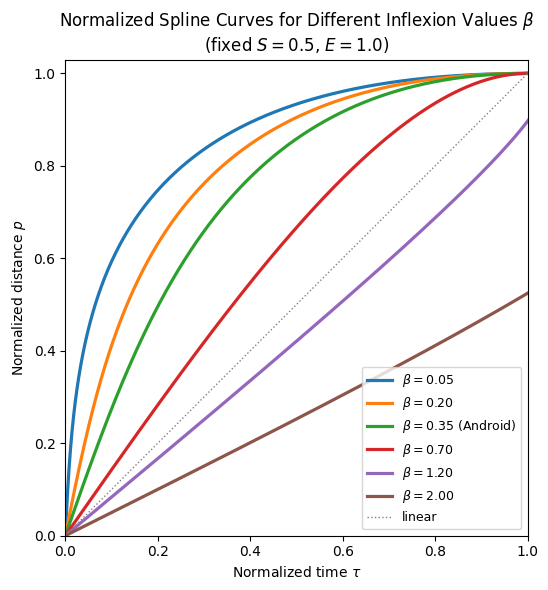
\includegraphics[width=0.7\textwidth]{../plots/Normalized_Spline_Curves_Plot.png}
        \caption{Normalized position-versus-time spline $p(\tau)$ for different inflexion values $\beta$, with the tension constants held fixed at $S=0.5$ and $E=1.0$. The Android default is $\beta=0.35$; the dotted diagonal marks the linear reference.}
        \label{fig:spline-beta}
        \end{figure}

        \chapter{System Description}

        \section{Overview and Design Rationale}

        The experimental system is a web-based apparatus for studying touch-driven list scrolling under a configurable transfer function. Its purpose is to present participants with a controlled search-and-select task on a long, continuously scrollable list, and to adapt the scrolling dynamics to each participant over the course of a session by means of an online optimization loop.

        The guiding architectural principle is a strict separation of concerns across three layers. A React single-page application presentation layer renders the list and takes full programmatic control of touch input and scrolling. A managed GraphQL API backed by a schemaless document store persistence layer records participants and their completed trial blocks. A serverless machine-learning backend optimization layer consumes the recorded data on demand and proposes the next transfer-function parameter set.

        A second, central design decision concerns the scrolling behaviour itself. Rather than relying on the browser's native momentum scrolling or on a framework's default scroll view, the post-touch (fling) motion is governed by an explicit, parameterized transfer function that was derived directly from the source code of Android's OverScroller class. Exposing the constants that are otherwise fixed in that source as tunable parameters turns regular preconfigured scrolling into a well-defined numerical search space, which the optimization layer can then adapt per participant. This coupling between a physically motivated interaction model and a data-driven optimizer is the conceptual core of the system.

        \section{System Architecture}

        The system is event-driven from end to end. Raw interaction data are recorded by the frontend, persisted in blocks of ten trials, evaluated on demand by a Gaussian-Process-based optimizer and the resulting new transfer-function parameters are made available to the participant for the subsequent block. The following subsections describe the four building blocks of this architecture.

        \subsection{Frontend}

        The frontend is a React single-page application written in plain JavaScript. Its static build artifacts (HTML, JavaScript, CSS) are hosted in an Amazon S3 bucket and delivered to participants through an Amazon CloudFront content-delivery distribution, which also terminates HTTPS. The frontend is responsible for rendering the list, running the custom touch-input and scrolling pipeline, evaluating the transfer function locally in real time, and collecting per-trial measurements that are submitted to the backend one block at a time.

        \subsection{Backend and Data Flow}

        The application backend is built around AWS AppSync, a managed GraphQL API service, which exposes queries and mutations for participant management, for storing completed trial blocks, and for requesting a new transfer-function parameter set. Amazon DynamoDB serves as the persistent, schemaless data store behind this API: each participant is represented as a single item holding the Prolific identifier, the demographic fields collected at registration (gender, smartphone model, handedness), the assigned study group, the currently active transfer-function parameter set, the next parameter set once available, the saved final (recommended) parameter set, and the complete history of completed trial blocks stored as a nested JSON attribute. Because a participant's entire state lives in one item, reading and appending trial data require no joins and remain a single-item operation.

        \subsection{Optimization Backend}

        The optimization backend is invoked synchronously as part of the GraphQL request flow. When a participant completes a block of trials, the frontend calls the mutation that requests the next parameter set. The AppSync resolver forwards this request to an AWS Lambda function, which reads that participant's stored block history from DynamoDB and sends it to an Amazon SageMaker inference endpoint that selects the parameters for the next block. Only the requesting participant's own data are used; the optimization is performed per participant rather than pooled across participants.

        The inference service is a stateless single-objective Bayesian optimizer. On each request, it reconstructs a per-participant training table from the incoming block-level observations, aggregates the ten trials of each block into a single scalar objective, the total length-normalized completion time, and fits a fresh Gaussian-process surrogate over the three-dimensional parameter space. While the model is still being learned, the next parameters are chosen by a noisy expected-improvement acquisition function; for the concluding recommendation, the model's posterior-mean optimum is returned instead.

        The resulting candidate parameter set is returned to the Lambda function, which writes it back to DynamoDB as the participant's next parameter set. The frontend then retrieves this value once the participant explicitly confirms readiness for the next block. This design keeps the optimization loop closed over the experimental data while maintaining a clear separation between data collection, inference, and the subsequent trial block.

        \subsection{Infrastructure as Code and Deployment}

        All infrastructure, the S3 bucket and CloudFront distribution, the AppSync API and its resolvers, the DynamoDB table, the Lambda function, and the SageMaker endpoint, is defined declaratively as code with Terraform and deployed through a GitHub Actions CI/CD pipeline. On every push to the main branch, the pipeline authenticates against AWS via OpenID Connect, runs terraform apply to reconcile the deployed AWS infrastructure with its version-controlled definition, and then builds and publishes the React frontend. This keeps the presentation, persistence, and optimization layers independently deployable while guaranteeing that the configuration used during data collection is fully reproducible from the repository.

        \section{Touch Input and Scrolling Pipeline}

        To obtain full and reproducible control over the scrolling dynamics, the frontend does not use the browser's native scrolling. Instead, it processes raw touch events and drives the list position programmatically, so that the fling behaviour is determined solely by the transfer function and not by browser or device-specific momentum implementations.

        \subsection{List and Scroll Container}

        The user interface presents a single continuously scrollable list of $N = 330$ entries, numbered consecutively. The list is not paginated in the sense of discrete page breaks or page-navigation controls. Instead, the height of each list entry is computed dynamically from the available viewport height so that exactly 15 entries are visible within the scroll container at any given time. This keeps the spatial density of the list, and therefore the visual arrangement participants perceive, consistent across devices and across trials.

        \subsection{Gesture Processing}

        The browser's and React's default scrolling behaviour is disabled for the list container and replaced by a custom pipeline that processes the native onTouchStart, onTouchMove, onTouchEnd, and onTouchCancel events directly. During a touch gesture, every touch-move sample is time-stamped and stored in a rolling buffer bounded by a $100$\,ms window and at most 20 samples. For real-time drag feedback the list follows the finger through an exponentially smoothed instantaneous velocity, while for launching a fling the release velocity is estimated from the buffered samples by a quadratic least-squares fit, taking the slope of the fitted curve at the moment of release as the launch velocity. This is more robust than a two-point derivative and, unlike a straight-line fit, follows the acceleration typically present at the end of a fling. If the estimated velocity exceeds a fixed fling threshold, it is clamped and passed into the fling model. Otherwise the list stops at its current position, after being clamped back into the valid scroll bounds if the participant had dragged past the list's edges.

        \subsection{Overscroll and Bounds Handling}

        Android's native scrolling system treats the list boundary as a special state. When a drag or fling would push the content beyond the valid range, the system allows a limited overscroll excursion and applies a resistance effect so that the visible motion decays smoothly near the boundary instead of abruptly stopping. Once the user releases the finger, or once the fling reaches the end of the valid range, the content is pulled back to the nearest legal position. This behavior is part of the general edge-response logic of the platform and is distinct from the actual fling trajectory itself: the ballistic motion is governed by the deceleration model, whereas the boundary handling is a separate mechanism that prevents the list from leaving its legal bounds.

        In this work, the same principle is implemented in a deliberately simplified form. The scroll position is always kept inside the valid list range, and any overshoot beyond the top or bottom is clamped and damped before being visualized. Unlike the full Android implementation, the project does not model the entire native edge state machine or its spring-back dynamics in detail; instead, it separates the concerns cleanly: the transfer function governs the in-bounds fling motion, while the bounds logic acts as a fixed, parameter-independent guard that stops the list at the valid edge and restores it to a legal position when necessary.

        \section{Adaptive Parameter Optimization}

        Trials are organized into blocks of 10, and a single transfer-function parameter set remains fixed for the duration of one block. After each block, the system may propose a new parameter set for the next block, gradually adapting the scrolling behaviour to the participant.

        \subsection{Warm-up and Bootstrap Phase}

        For the first three blocks of each participant, the machine-learning backend is not yet used to propose parameters. Instead, each parameter is independently sampled uniformly at random from its predefined bounds. This warm-up/bootstrap phase serves two purposes: it generates an initial, sufficiently diverse set of observations for the optimization model to learn from, and it avoids relying on an uninitialized or poorly informed model at the very beginning of a session, where no data are yet available.

        \subsection{Model-Based Optimization per Participant}

        Only after these first three blocks have been completed does the system switch to model-based parameter generation. In contrast to a pooled, cross-participant scheme, the optimization is carried out \emph{per participant}: whenever a new parameter set is requested, the Lambda function retrieves only the requesting participant's completed block histories and forwards them to the SageMaker endpoint. No data from other participants and no participant-identity feature enter the model.

        Each recorded trial contains the completion time \texttt{timeMs}, the target index \texttt{targetNumber}, the block index \texttt{blockIndex}, and the transfer-function parameters active for that block in \texttt{paperParams}. On the inference side, the trials are grouped by block; the parameter vector is taken from the block's parameter set, and the ten trials of a block are aggregated into a single scalar objective, the total length-normalized completion time. Each trial time is divided by its target index, which is proportional to the required scroll distance, and summed over the block, so that near and far targets contribute comparably. This yields one observation per block,
        \begin{equation}
            x = [\mu,\ r,\ \beta] \;\longrightarrow\; y = \sum_{k=1}^{10} \frac{t_k}{n_k},
            \label{eq:sd-scalar-objective}
        \end{equation}
        where $t_k$ is the completion time and $n_k$ the target index of the $k$-th trial in the block. Minimizing $y$ rewards parameter sets that let the participant reach the targets quickly across the whole list.

        A single-output Gaussian process (\texttt{SingleTaskGP}) is fitted to these block observations. Inputs are mapped to the unit cube by a \texttt{Normalize} input transform over the fixed parameter bounds, and the objective is standardized by a \texttt{Standardize} outcome transform; the kernel and observation-noise hyperparameters are then learned by maximizing the marginal log-likelihood. Because the noise level is inferred during fitting, no manual noise floor, covariance jitter, or duplicate collapsing is applied; the implementation relies on the numerically stable BoTorch fitting routine instead. As BoTorch maximizes by convention, the negative normalized time is used as the internal objective.

        \subsection{Optimization Schedule and Counterbalancing}

        Parameter generation follows a fixed schedule of fifteen blocks per participant. The first three blocks are the random warm-up described above. Blocks four to thirteen constitute the optimization phase: for each of them the Gaussian process is refitted on all preceding blocks, and the next parameter set is proposed with the numerically stable noisy expected-improvement acquisition function (qLogNEI), which balances exploration and exploitation while the model is still being learned.

        Training is deliberately frozen after block thirteen. The two final blocks, fourteen and fifteen, no longer contribute to the model; they form a within-participant comparison between the learned transfer function and the original Android defaults. Once block thirteen is complete, the model's final recommendation is computed once, from the thirteen training blocks only, as the minimizer of the posterior mean (the \texttt{PosteriorMean} criterion, i.e.\ the parameter set that the fitted model predicts to be fastest), and is stored with the participant. Whichever of the two final blocks is the learned-parameter block then loads this saved recommendation instead of triggering a further optimization run, which guarantees that the Android block's measurements can never enter the training data.

        Which of the two final blocks uses the learned parameters and which uses the Android defaults is counterbalanced across participants by a study-group assignment passed as a URL parameter. In one group the learned recommendation is presented as block fourteen and the Android defaults as block fifteen; in the other group the order is reversed. This ordering variable is stored with the participant so that potential order effects can be accounted for in the analysis.

        \subsection{SageMaker Inference Implementation and Deployment}

        The inference logic is implemented as a single stateless Python module exposing the required SageMaker entry points \texttt{model\_fn}, \texttt{input\_fn}, \texttt{predict\_fn}, and \texttt{output\_fn}. \texttt{model\_fn} returns an essentially empty handle, while data preparation, Gaussian-process fitting, acquisition optimization, and response packaging are all performed inside \texttt{predict\_fn}. A fresh model is fitted on every invocation from the current payload, which keeps the deployment stateless and guarantees that each proposal reflects the participant's most recent data.

        Given the fitted model, the next parameter vector is obtained by maximizing the selected acquisition function over the box-constrained space with BoTorch's \texttt{optimize\_acqf}, starting from several quasi-random restarts. During the optimization phase this acquisition is qLogNEI; for the final recommendation it is the posterior mean. Unlike the earlier implementation, no discrete candidate grid or probe ranking is used: the continuous optimizer returns a point in parameter space directly, which is then clipped to the bounds and quantized to the parameter-specific precision. If fewer than two block observations are available, the endpoint declines to fit a model, and the surrounding Lambda logic falls back to the participant's current parameters. The response is exchanged as \texttt{application/json} and contains the chosen parameter vector together with a concise diagnostic bundle (the acquisition strategy and value, the number of training blocks, and the best observed normalized time).

        The module is packaged with its runtime files into a gzip-compressed \texttt{model.tar.gz} in SageMaker's \texttt{code/} layout, uploaded to S3 by Terraform, and loaded into a prebuilt PyTorch inference container via the \texttt{SAGEMAKER\_PROGRAM} and \texttt{SAGEMAKER\_SUBMIT\_DIRECTORY} environment variables, since the Gaussian-process model and the acquisition functions depend on the PyTorch and BoTorch backend. The shared parameter-bounds file is packaged alongside the inference code, so that the endpoint enforces exactly the same search space as the frontend.

        \chapter{Experimental Procedure}
        \label{sec:procedure}

        \section{Recruitment and Onboarding}

        Participants were recruited through the Prolific crowdsourcing platform and opened the study via a personalized link that carries their Prolific identifier and a study-group assignment as URL parameters. On entry, they are shown an information and informed-consent screen that states the purpose of the study, the expected duration, the eligibility requirements, the data that are recorded, and a contact address; participation continues only after the participant actively confirms consent. Only iPhone devices are admitted, so that the display density, and hence the physical scrolling coefficient $C$ of Equation~\eqref{eq:sd-physical-coeff}, is held constant across participants. A short registration form then records three demographic items, gender, smartphone model, and handedness, before the task begins. After the final block, participants are redirected back to Prolific through a completion URL that registers the submission.

        \section{Pilot Study and Participants}

        Prior to the main data collection, a small pilot study was carried out to calibrate the parameter search space. Three participants completed the full procedure with the initial, deliberately wide parameter bounds. Their recorded behaviour was used to decide how to constrain the bounds of the fling-friction, deceleration-rate, and inflexion parameters for the main study, so that the admissible transfer functions remain usable while still spanning a meaningful range of scrolling dynamics.

        The main study was then conducted with 32 participants recruited through Prolific, balanced by gender with 16 women and 16 men.

        \section{Task Design}
        \label{sec:task}

        Participants were asked to repeatedly locate and select a specified target entry within the 330-entry list. Ten fixed target positions were used throughout the experiment: entries $30, 60, 90, \dots, 300$, i.e.\ every 30th position starting 30 entries from the top and ending 30 entries from the bottom of the list. This excludes the first and last 30 entries from ever being used as a target, so that every target position is reachable by scrolling in either direction and no target is trivially visible without scrolling.

        For each block of trials -- corresponding to one fixed transfer-function parameter set -- all 10 target positions were presented exactly once, in a randomized order that was freshly shuffled at the start of every block. Before the first randomized block, participants completed a single untimed practice trial with a fixed target (list entry 180) in order to familiarize themselves with the touch-scrolling interaction and the location-feedback display; this practice trial is not included in the recorded/optimized trial data.

        \section{Interface Elements and Progress Feedback}
        \label{sec:interface}

        A horizontal progress indicator above the list shows, as a row of 10 pill-shaped segments, how many of the 10 trials belonging to the currently active transfer function have already been completed. Directly above the list, a banner displays the number the participant is currently searching for. Two identical vertical location-feedback tracks are rendered on the left and right edge of the screen, each showing two markers: one fixed at the position of the current target (proportional to its index within the 330-entry list) and one continuously updated to reflect the participant's current scroll position (computed from the on-screen offset of the topmost rendered items). This lets participants continuously orient themselves relative to the target without having to keep the target itself in view while scrolling. While a trial is in progress, the target entry is visually distinguished from all other (otherwise identically styled) entries by a red border and light red background; once the participant has tapped the correct entry, it briefly switches to a green background before the next trial begins.

        \section{Data Collection and Recorded Metrics}
        \label{sec:data-collection}

        In addition to the timing data used by the optimizer, several gesture-level quantities are computed in real time during each trial for on-screen feedback and threshold-logic purposes, including swipe direction, per-gesture distance and duration, average and maximum swipe speed, the number of direction reversals (``switchbacks''/clutches) within a trial, and whether and by how far the target was overshot. Of these, the total elapsed time until the correct entry is tapped (\texttt{timeMs}), the net scrolled distance during the trial (\texttt{scrollDistance}), and a completion timestamp are recorded and persisted to the backend per trial; the completion time forms the basis of the block-level optimization objective of Equation~\eqref{eq:sd-scalar-objective}.

        Trial data belonging to one block are collected locally in the browser and only submitted to the backend once all 10 trials of a block are complete, at which point they are appended atomically to the participant's stored trial history together with the transfer-function parameter set that was active during that block. After a block has been submitted, the list is covered by a waiting overlay showing a circular progress indicator until a new parameter set has been generated, either by random sampling during the warm-up phase, by the Gaussian-process optimizer during the optimization phase, or by loading the stored recommendation or the Android defaults for the two final blocks. The overlay is lifted automatically once the new transfer function is active, at which point the next block begins. This creates a clear separation between successive blocks and ensures that a new transfer function is only introduced once the backend has produced a validated parameter set.

        \chapter{Results and/or Evaluation}

        This chapter evaluates whether the per-participant optimized transfer function improves scrolling performance over Android's default function. The evaluation rests on the within-participant comparison built into the study design: the two final blocks present, in counterbalanced order, once the learned recommendation (the \emph{optimized} condition) and once the unmodified Android defaults (the \emph{Android} condition), so that every participant contributes one block under each condition. Three questions are addressed in turn: (i) does the optimized function outperform the Android default across all participants; (ii) does this effect differ between women and men; and (iii) how does the comparison depend on the scrolling distance to the target.

        \section{Outcome Measure and Analysis Approach}

        The primary outcome is the completion time of a trial, i.e.\ the elapsed time \texttt{timeMs} from the appearance of a target until the correct list entry is tapped. Because the ten targets of a block lie at systematically different distances, raw times are not directly comparable across trials; the length-normalized time
        \begin{equation}
        \hat{t}_{i} \;=\; \frac{t_i}{n_i},
        \label{eq:eval-normalized-time}
        \end{equation}
        where $t_i$ is the completion time and $n_i \in \{30,60,\dots,300\}$ the target index (proportional to the required scroll distance), is used as the distance-invariant performance measure, consistent with the optimization objective of Equation~\eqref{eq:sd-scalar-objective}. For the aggregate analyses, each participant contributes a single value per condition, obtained by averaging $\hat{t}_i$ over the ten trials of the respective block.

        Analysis proceeds in two stages, following common practice for pointing- and scrolling-style tasks. First, an \emph{error rate} is computed as the proportion of trials in which the target was overshot at least once (\texttt{didOvershoot}); trials are additionally screened for extreme outliers in completion time, which are removed before the timing analysis. Second, the timing comparison is carried out on the cleaned data. Because the design is within-participant, all condition comparisons are paired; normality of the paired differences is checked, and a paired $t$-test is used when it is tenable and the Wilcoxon signed-rank test otherwise. Effect sizes (Cohen's $d_z$ or the rank-biserial correlation) and the counterbalancing order are reported so that potential order effects can be ruled out.

        \section{Statistical Methods and Robustness Checks}

        Because the tests differ in whether they compare \emph{paired} (within-participant) or \emph{independent} (between-group) samples, the appropriate procedure is chosen per question rather than applying a single test throughout. The Android-versus-optimized contrast is inherently paired, since each participant provides one block per condition, so it is analysed with the Wilcoxon signed-rank test (or a paired $t$-test when the paired differences are approximately normal). Comparisons \emph{between} the two gender groups are independent and therefore use the Mann-Whitney $U$ test, applied to the per-participant improvement $\Delta=\hat{t}_{\text{opt}}-\hat{t}_{\text{And.}}$; a mixed analysis of variance provides the equivalent parametric account through its \emph{Function}~$\times$~\emph{Gender} interaction. Categorical outcomes are treated analogously: a $2\times 2$ table of independent counts, such as the number of participants for whom the optimized function was faster split by gender, is assessed with Fisher's exact test, whereas a paired binary outcome, such as whether a participant overshot more often under one condition than the other, is assessed with McNemar's test.

        The distance-resolved analysis warrants particular care, because each participant contributes only a single trial per condition and distance, leaving no within-cell replication. In addition to the $2\times 10$ repeated-measures analysis of variance, the same data are therefore modelled with a linear mixed-effects model with fixed effects for \emph{Function}, \emph{Distance}, and their interaction and a random intercept per participant, which handles the nesting of trials within participants without requiring aggregation. The trial-level secondary measures (overshoots, direction reversals) are similarly non-independent and are either aggregated to one value per participant and condition before a paired test, or modelled with a generalised linear mixed-effects model with a per-participant random intercept.

        The reported conclusions are supported by the following robustness checks:
        \begin{itemize}
        \item \emph{Distribution-free confirmation.} Every paired comparison is repeated with a paired sign-flip permutation test ($10^4$ Monte Carlo resamples), and each between-group comparison with a label-shuffle permutation test, so that the conclusions do not rest on a distributional assumption.
        \item \emph{Parametric versus non-parametric.} Paired $t$-test and Wilcoxon results are reported side by side; agreement between them indicates that the choice of test does not drive the conclusion.
        \item \emph{Aggregation and outliers.} Results are recomputed using the per-participant median instead of the mean, and with and without the removed completion-time outliers (flagged per participant/distance rather than globally), to confirm that neither choice materially changes the outcome.
        \item \emph{Order effects.} The counterbalancing group (block order) is added as a factor to verify that the effect of \emph{Function} is not confounded with presentation order or carry-over.
        \item \emph{Effect sizes with uncertainty.} Alongside $p$-values, standardized effect sizes (Cohen's $d_z$; rank-biserial correlation) and $95\%$ bootstrap confidence intervals for the mean difference and the percentage improvement are reported, which is especially important given the moderate sample size ($n=\evalval{nParticipants}$; \evalval{nFemale} women and \evalval{nMale} men), where the \emph{Function}~$\times$~\emph{Gender} interaction is only modestly powered and is therefore treated as exploratory.
        \item \emph{Multiple comparisons.} Where a family of tests is run, in particular across the ten target distances and the secondary measures, $p$-values are corrected with the Holm or Benjamini-Hochberg procedure, and a single primary outcome (the overall paired time comparison) is distinguished in advance from the exploratory analyses.
        \end{itemize}
        Finally, the overshoot-based ``error rate'' is a proxy for accuracy rather than a count of mis-taps, since the task requires tapping the correct entry to proceed and wrong taps are not separately recorded; it is interpreted accordingly.

        \section{Overall Comparison: Android vs.\ Optimized}

        The first analysis pools all \evalval{nParticipants} participants and compares the mean length-normalized time of the optimized condition against the Android condition. Figure~\ref{fig:eval-overall} contrasts the two conditions, and Table~\ref{tab:eval-overall} reports the paired difference together with its effect size and significance. A negative difference (optimized minus Android) indicates that the learned function let participants reach the targets faster than the Android default. The same paired test is applied to the secondary measures, the overshoot-based error rate and the number of direction reversals (\texttt{switchbackCount}), to check whether any timing gain is accompanied by more or fewer corrective movements.

        Across the \evalval{nParticipants} participants, the optimized function lowered the mean length-normalized time from \evalval{overallAndroidMean} to \evalval{overallOptimizedMean}\,ms/index, a paired difference of \evalval{overallDiff}\,ms/index (\evalval{overallPctImprovement}\,\% faster; $95\%$ bootstrap CI $[\evalval{overallCiLow},\,\evalval{overallCiHigh}]$; Cohen's $d_z=\evalval{overallCohenDz}$; paired $t$-test $p=\evalval{overallTp}$, Wilcoxon $p=\evalval{overallWilcoxonP}$, sign-flip permutation $p=\evalval{overallPermP}$).

        \begin{figure}[htbp]
        \centering
        \includegraphics[width=0.7\textwidth]{eval_android_vs_optimized_overall.png}
        \caption{Mean length-normalized completion time under the Android and the optimized transfer function, aggregated over all participants. Error bars denote the standard error of the paired means.}
        \label{fig:eval-overall}
        \end{figure}

        \begin{table}[htbp]
        \centering
        \begin{tabular}{l r r r r}
        \hline
        Measure & Android & Optimized & $\Delta$ (Opt.$-$And.) & $p$ \\
        \hline
        Norm.\ time (ms/index) & \evalval{overallAndroidMean} & \evalval{overallOptimizedMean} & \evalval{overallDiff} & \evalval{overallWilcoxonP} \\
        Error rate (overshoot) & \evalval{errAndroid} & \evalval{errOptimized} & \evalval{errDiff} & \evalval{errWilcoxonP} \\
        Switchbacks per trial   & \evalval{swAndroid} & \evalval{swOptimized} & \evalval{swDiff} & \evalval{swWilcoxonP} \\
        \hline
        \end{tabular}
        \caption{Overall within-participant comparison of the Android and optimized conditions (means over all participants). All values are read from \texttt{eval\_results.csv}; $p$ is the Wilcoxon signed-rank result.}
        \label{tab:eval-overall}
        \end{table}

        \section{Comparison by Gender}

        Because the sample is split by gender (\evalval{nFemale} women, \evalval{nMale} men), the same paired comparison is repeated separately within each group, and the two effects are contrasted. This is formalized as a $2\times 2$ mixed analysis of variance with the within-participant factor \emph{Function} (Android vs.\ optimized) and the between-participant factor \emph{Gender} (female vs.\ male). The main effect of \emph{Function} quantifies the overall benefit of optimization, the main effect of \emph{Gender} captures baseline differences in scrolling speed, and the \emph{Function}~$\times$~\emph{Gender} interaction indicates whether the optimization benefits one group more than the other. Figure~\ref{fig:eval-gender} shows the two conditions side by side for women and men, and Table~\ref{tab:eval-gender} reports the per-group paired differences. The between-group difference in the per-participant improvement $\Delta$ is assessed with the Mann-Whitney $U$ test ($p=\evalval{mannwhitneyDeltaP}$).

        \begin{figure}[htbp]
        \centering
        \includegraphics[width=0.8\textwidth]{eval_android_vs_optimized_by_gender.png}
        \caption{Mean length-normalized completion time under the Android and optimized functions, separately for female and male participants. Error bars denote the standard error of the means.}
        \label{fig:eval-gender}
        \end{figure}

        \begin{table}[htbp]
        \centering
        \begin{tabular}{l r r r r}
        \hline
        Group & Android & Optimized & $\Delta$ (Opt.$-$And.) & $p$ \\
        \hline
        Women ($n=\evalval{genderFemaleN}$) & \evalval{genderFemaleAndroid} & \evalval{genderFemaleOptimized} & \evalval{genderFemaleDiff} & \evalval{genderFemaleWilcoxonP} \\
        Men ($n=\evalval{genderMaleN}$)   & \evalval{genderMaleAndroid} & \evalval{genderMaleOptimized} & \evalval{genderMaleDiff} & \evalval{genderMaleWilcoxonP} \\
        \hline
        \end{tabular}
        \caption{Within-participant Android-vs-optimized comparison of the mean length-normalized time, separately by gender. The Function\,$\times$\,Gender interaction from the mixed ANOVA is reported in the text.}
        \label{tab:eval-gender}
        \end{table}

        \section{Comparison by Target Distance}

        The aggregate measures may mask distance-dependent effects, since near and far targets stress the fling behaviour differently. Each block contains exactly one trial per target position, so every participant contributes one completion time per condition and per distance $n \in \{30,60,\dots,300\}$. For this analysis the raw completion time $t_i$ (rather than the normalized $\hat{t}_i$) is used, because distance is now an explicit factor rather than something to be normalized away. The comparison is modelled as a $2\times 10$ repeated-measures analysis of variance with the within-participant factors \emph{Function} (Android vs.\ optimized) and \emph{Distance} (the ten target positions). The main effect of \emph{Distance} is expected to be large and merely confirms that farther targets take longer; the effect of interest is the \emph{Function}~$\times$~\emph{Distance} interaction, which reveals whether the optimized function's advantage is concentrated at short, medium, or long distances. Figure~\ref{fig:eval-distance} plots completion time against target distance for both conditions. The repeated-measures ANOVA reports a \emph{Distance} main effect ($F=\evalval{rmanovaDistanceF}$, $p=\evalval{rmanovaDistanceP}$), a \emph{Function} effect ($F=\evalval{rmanovaConditionF}$, $p=\evalval{rmanovaConditionP}$), and a \emph{Function}~$\times$~\emph{Distance} interaction ($F=\evalval{rmanovaInteractionF}$, $p=\evalval{rmanovaInteractionP}$); the linear mixed-effects model yields a matching interaction coefficient of \evalval{lmmInteractionCoef}\,ms/index ($p=\evalval{lmmInteractionP}$).

        \begin{figure}[htbp]
        \centering
        \includegraphics[width=0.8\textwidth]{eval_android_vs_optimized_by_distance.png}
        \caption{Mean completion time as a function of target distance (index $30,60,\dots,300$) under the Android and optimized transfer functions, aggregated over all participants. Error bars denote the standard error of the means.}
        \label{fig:eval-distance}
        \end{figure}

        Finally, the distance-resolved comparison is broken down by gender, yielding the same distance profiles separately for women and men (Figure~\ref{fig:eval-distance-gender}). This corresponds to a three-factor design with the within-participant factors \emph{Function} and \emph{Distance} and the between-participant factor \emph{Gender}, and it indicates whether any gender difference in the optimization benefit is uniform across distances or specific to particular scroll lengths.

        \begin{figure}[htbp]
        \centering
        \includegraphics[width=0.9\textwidth]{eval_android_vs_optimized_by_distance_gender.png}
        \caption{Mean completion time versus target distance under the Android and optimized functions, separately for female and male participants.}
        \label{fig:eval-distance-gender}
        \end{figure}

        \section{Parameter Influence on Performance}

        The optimized transfer functions differ from one another in three correlated parameters, the fling friction $\mu$, the deceleration rate $r$, and the inflexion $\beta$. To quantify how each of them affects performance, \emph{all} blocks of \emph{all} participants are pooled: every block contributes one parameter vector $[\mu,\ r,\ \beta]$ and the mean length-normalized time achieved under it (lower is better). Because the three parameters differ in scale and range, both the parameters and the outcome are standardized to zero mean and unit variance, and a linear mixed-effects model $z(\hat{t}) \sim z(\mu)+z(r)+z(\beta)$ with a per-participant random intercept is fitted. The standardized coefficients are therefore directly comparable in magnitude, and a negative sign means that a larger value of that parameter shortens the completion time.

        The largest influence is exerted by the deceleration rate $r$ (standardized $\beta=\evalval{inflDecelerationRateBeta}$, $p=\evalval{inflDecelerationRateP}$), followed by the inflexion $\beta$ ($\evalval{inflInflexionBeta}$, $p=\evalval{inflInflexionP}$) and the fling friction $\mu$ ($\evalval{inflScrollFrictionBeta}$, $p=\evalval{inflScrollFrictionP}$). Figure~\ref{fig:eval-param-influence} shows these coefficients and Table~\ref{tab:eval-influence} lists them together with the pooled Spearman correlations, while Figure~\ref{fig:eval-param-marginal} shows the marginal relationship between each parameter and the achieved time, revealing whether the effect is monotone or has an interior optimum.

        \begin{figure}[htbp]
        \centering
        \includegraphics[width=0.7\textwidth]{eval_param_influence.png}
        \caption{Standardized effect of each parameter on the length-normalized completion time (pooled over all blocks and participants, with a per-participant random intercept). A negative coefficient means that increasing the parameter reduces completion time (better).}
        \label{fig:eval-param-influence}
        \end{figure}

        \begin{table}[htbp]
        \centering
        \begin{tabular}{l r r r}
        \hline
        Parameter & Std.\ $\beta$ & $p$ & Spearman $\rho$ \\
        \hline
        $\mu$ (scrollFriction) & \evalval{inflScrollFrictionBeta} & \evalval{inflScrollFrictionP} & \evalval{spearmanScrollFriction} \\
        $r$ (decelerationRate) & \evalval{inflDecelerationRateBeta} & \evalval{inflDecelerationRateP} & \evalval{spearmanDecelerationRate} \\
        $\beta$ (inflexion) & \evalval{inflInflexionBeta} & \evalval{inflInflexionP} & \evalval{spearmanInflexion} \\
        \hline
        \end{tabular}
        \caption{Influence of each transfer-function parameter on the length-normalized completion time. Standardized mixed-model coefficients (negative $=$ faster) and pooled Spearman correlations, read from \texttt{eval\_results.csv}.}
        \label{tab:eval-influence}
        \end{table}

        \begin{figure}[htbp]
        \centering
        \includegraphics[width=0.9\textwidth]{eval_param_marginal_effects.png}
        \caption{Marginal relationship between each parameter value and the block-mean length-normalized time (scatter over all blocks, with a low-order polynomial fit and binned means). The dotted line marks the Android default.}
        \label{fig:eval-param-marginal}
        \end{figure}

        \section{Does Personalization Pay Off?}

        A central premise of this work is that the transfer function is optimized \emph{per participant} rather than fitted once for the whole population. Whether this personalization is warranted depends on how much the learned optima actually differ between participants: if every participant converges to a similar parameter vector, a single pooled function would suffice and the per-participant machinery adds little; if the optima are widely dispersed, personalization is justified because no single function can serve everyone well. This question is therefore examined by quantifying the spread of the optimized parameters across participants and by relating it to the width of the admissible search space.

        For each of the three free parameters the distribution of the learned values across the \evalval{nParticipants} participants is summarized (median, interquartile range, and full range), and its dispersion is expressed relative to the corresponding bound of the search space, e.g.\ the interquartile range of $\mu$ as a fraction of $[0.0025,0.2]$. A parameter whose optima cluster tightly within a small sub-interval indicates population-level agreement, whereas one that spreads across a large share of its admissible range indicates genuine inter-individual differences that only personalization can accommodate. Concretely, the interquartile range spans \evalval{spreadScrollFrictionIqrPct}\,\% of the admissible interval for $\mu$, \evalval{spreadDecelerationRateIqrPct}\,\% for $r$, and \evalval{spreadInflexionIqrPct}\,\% for $\beta$. Figure~\ref{fig:eval-param-spread} shows the per-parameter distributions of the optimized values together with the Android default as a reference line.

        \begin{figure}[htbp]
        \centering
        \includegraphics[width=0.8\textwidth]{eval_optimized_param_spread.png}
        \caption{Distribution of the optimized parameter values $\mu$, $r$, and $\beta$ across the \evalval{nParticipants} participants (box-and-whisker over the admissible range of each parameter). The dashed line marks the Android default; wide dispersion relative to the search-space bounds indicates that personalization is warranted.}
        \label{fig:eval-param-spread}
        \end{figure}

        As a descriptive counterfactual, a single \emph{pooled} function is constructed from the element-wise median of the optimized parameter vectors, $[\tilde{\mu},\tilde{r},\tilde{\beta}]$, and its distance to each participant's own optimum is reported. Here $[\tilde{\mu},\tilde{r},\tilde{\beta}]=[\evalval{pooledMedianScrollFriction},\,\evalval{pooledMedianDecelerationRate},\,\evalval{pooledMedianInflexion}]$, and the individual optima lie at a mean normalized distance of \evalval{pooledDistMean} (at most \evalval{pooledDistMax}) from this pooled vector. Large per-participant deviations from this pooled vector would indicate that a one-size-fits-all function is a poor substitute for the personalized one. It must be stressed, however, that this comparison is necessarily \emph{descriptive}: because each participant provides completion times only for their own learned function and the Android default, the study contains no measurements of how a participant would have performed under the pooled function. A rigorous pooled-versus-personalized performance comparison would require either a further experimental condition in which the pooled function is presented, or a predictive simulation that estimates each participant's time under the pooled parameters from their fitted surrogate model; both are left to future work. The present analysis therefore establishes only whether the \emph{parameters} justify personalization, not the magnitude of the performance loss a pooled function would incur.

        %%%%%%%%%%%%%%%%%%
        \chapter{Conclusion and Future Work}

        \section*{Key Insights}

        Discuss key findings and their implications.

        \section*{Future Directions}

        Provide suggestions for future work and potential applications.

        %%%%%%%%%%%%%%%%%%
        \chapter{Availability}

        This chapter is optional. If the thesis has lead to the generation of data, or to the implementation of software, or to a manuscript
        or publication, then where can it be obtained from?

        %%%%%%%%%%%%%%%%%%
        \chapter*{References}
        \addcontentsline{toc}{chapter}{References}
        \bibliographystyle{plainnat}
        \bibliography{bibliography}

        %%%%%%%%%%%%%%%%%%
        \appendix
        \chapter{Appendix Title}
        Include any additional material, such as data, code, or supplementary figures.

        %%%%%%%%%%%%%%%%%%
        \selectlanguage{ngerman}
        \chapter*{Selbstst\"andigkeitserkl\"arung}
        \addcontentsline{toc}{chapter}{Selbstst\"andigkeitserkl\"arung}

        Bitte  die ``Erkl\"arung Abschlussarbeit (PDF) (f\"ur Abschlussarbeiten in allen B.Sc./M.Sc.-Studieng\"angen am FB Informatik inklusive B.Ed./M.Ed. Informatik)'',
        auf den Webseiten des Fachbereiches erh\"altlich, \url{https://uni-tuebingen.de/de/74351},
        ausf\"ulen, unterschreiben und hier anh\"angen.

        \end{document}